Ever since ancient Greece, people have been trying to discover what makes up everything. Empedocles, an ancient Greek philosopher, said that everything was comprised of four elements: earth, fire, water, and air. Although modern scientists use more than four elements, they are still trying to categorize the most fundamental substance. Democritus proposed that everything, if divided enough times, could be broken down into atoms at their most fundamental level. While the term ``atom'' came to be known for something that was not the most fundamental substance, scientists today are still pursuing the ``atom'' theorized by Democritus.

In the 19th century, John Dalton believed he found the most fundamental particle and named it the atom, but as time passed, there was strong evidence that even atoms had internal components and structure. This was proven when J.~J.~Thompson in the late 19th century found the electron, which proved to be a component of the atom. The electron was not only the first fundamental particle discovered, but also the beginning of particle physics as a field of study. While it was an insightful discovery that led to many inventions, there were still many unknowns about the atom. About a decade after Thompson, Robert Millikan made fine measurements of the charge and mass of the electron, but this raised even more questions about the atom. In the early 20th century, Ernest Rutherford showed that the atom is mostly empty space with a very dense core called the nucleus, which has a charge opposite to that of the electron. In his experiment, Rutherford shot alpha particles, made up of two protons and two neutrons, at gold foil and observed their scattering angle. Most of the alpha particles passed through unperturbed, but a handful were significantly deflected. From this observation, Rutherford concluded that most of the atom is empty space while having a highly dense core called the nucleus. 

These discoveries showed that there were more things to explore beyond the atom. In parallel, there were equally important theories being developed. Quantum mechanics is essential to the study of sub-atomic particles as they no longer behave according to classical mechanics. During this development Max Planck was doing his work on the quantization of energy. This set the groundwork for quantum mechanics and also served as a basis to Einstein's work. Einstein formulated the important concept of light as a particle called the photon. Previously, light had been described as a wave, but Einstein showed that light had many particle-like properties including momentum. This theory and the more traditional view of light as a wave were combined leading to the wave particle duality of light. Eventually Louis De Brogile extended this duality to all particles theorizing that all particles including electrons and other sub-atomic particles could be described using waves or particles.

Einstein's theory of relativity had another major impact on particle physics. The most famous of Einstein's equation, $E = mc^2$, shows the mass-energy relationship. One of the implications of quantum mechanics is that if something can happen it will happen under a certain probability. This means that given the right conditions and enough energy, one can create mass. There are other conservation laws which need to be followed and are still relevant to particle physics, but conservation of energy is one of the biggest limiters. In order to create more massive particles, more energy is needed. 

As these theories became more complete, they supplied a more complete picture of these subatomic particle, such as the electron states and the protons and neutrons in the nucleus of the atom. Scientist also began to find evidence of fundamental particles not in atoms. In 1932 Carl Anderson found evidence of a muon from cosmic rays. In addition, as scientists began to probe higher energies, they found evidence of internal structure within protons and neutrons. In 1968 at the Standford Linear Accelerator Center, they found evidence of particles within protons, which were later called quarks.

The discovery of more and more fundamental particles led to the formulation of the standard model. The two main groups of particles in the standard model are fermions, which have half integer spin, and bosons, which have integer spin. The main physical difference this causes comes from the Pauli exclusion principle, which allows fermions to build into larger arrangements. Because of this fermions are the building blocks of the macroscopic world as they make up protons, neutrons, and also atoms.   

As shown in table~\ref{tab:particles} there are several different groups of particles in the standard model. The first group is a sub-category of fermions called quarks. The main factor that distinguishes quarks from other fundamental fermions is that they interact via the strong force. While they also interact via the electromagnetic and weak forces, the strong force is the dominate one. Quarks can exist in isolation only for a short time, and they quickly recombine in groups of two, three, or possibly more. When three quarks form a particle it is called a baryon. A proton, which is made up of two up quarks and one down quarks, and a neutron, which is made up of two down and one up quarks, are both baryons. Each of the quarks inside a baryon has a different color --- red, green, or blue --- which serves as the ``charge'' for the strong force. Similar to electric charge, strong force color attracts other colors and repels similar colors, but since the baryon has one of each it has a net color of white or nothing. In addition to the six flavors of quark listed in table~\ref{tab:particles}, there is also a corresponding antiquark with the same properties but opposite charge and color. Quark and antiquark pairs can form color neutral particles called mesons. If one tries to separate the individual quarks from the respective baryons or mesons the energy required to separate them is more than the energy required to create more quarks. For instance, when the constituent quarks in a proton are being pulled apart, there comes a point when the energy used to separate them is sufficient to create more quarks. This energy will be used to create new quarks leaving no quarks in isolation.

The other category of fermionic particles is leptons. Unlike the quarks, leptons are not affected by the strong force, and therefore it is more common to find them in isolation. The electron is the most well-known lepton, but there are also two other flavors which are heavier copies of the electron. As with all of the particles in the standard model, there are corresponding antiparticles for the each lepton with the same mass but opposite charge. In addition to the three charged leptons, there are also three neutral leptons, which are called neutrinos. Each one has a charged lepton partner. Neutrinos are nearly massless and do not have any charge. Since the only force that affects them is the weak force, they have a very low probability of interaction. This means that they essentially pass through everything without interaction. Although they do interact through processes such as beta decay, most neutrinos simply travel through everything. 

Finally, there are the bosons. Bosons are different from both leptons and quarks in that they have integer spin, but the individual bosons differ from each other in which fundamental force affects them. While leptons and quarks combine together to form complex arrangements such as atoms and all of matter, bosons serve as the force carriers. The photon serves as the mediator for the electromagnetic force, which means that whenever two electrons repel each other there is a photon to mediate that interaction. The strong force interaction is mediated by the gluon. The weak force is mediated by the W boson, for those interactions with changes in charge, and the Z boson, for those interactions with no changes in charge. 

\begin{table}
\caption{Particles in the Standard Model~\cite{pdg}}
\label{tab:particles}
\begin{center}
\begin{tabular}{|c|c|c|c|c|}
\hline
Particle Type & Name & Charge & Mass & Spin \\
\hline
\multirow{6}{*}{Quarks} & Up & $+2/3e$ & $2.2\MeVcc$ & $\pm 1/2$ \\
& Down & $-1/3e$ & $4.7\MeVcc$ & $\pm 1/2$ \\
& Charm & $+2/3e$ & $1.28\GeVcc$ & $\pm 1/2$ \\
& Strange & $-1/3e$ & $96\MeVcc$ & $\pm 1/2$ \\
& Top & $+2/3e$ & $173.1\GeVcc$ & $\pm 1/2$ \\
& Bottom & $-1/3e$ & $4.18\GeVcc$ & $\pm 1/2$ \\
\hline
\multirow{6}{*}{Leptons} & Electron & $-1e$ & $0.511\MeVcc$ & $\pm 1/2$ \\
& Muon & $-1e$ & $105.7\MeVcc$ & $\pm 1/2$ \\
& Tau & $-1e$ & $1.776\GeVcc$ & $\pm 1/2$ \\
& Electron Neutrino & $0$ & $\approx 0$ & $\pm 1/2$ \\
& Muon Neutrino & $0$ & $\approx 0$ & $\pm 1/2$ \\
& Tau Neutrino & $0$ & $\approx 0$ & $\pm 1/2$ \\
\hline
\multirow{4}{*}{Gauge Bosons} & Photon & 0 & 0 & $\pm 1$ \\
& Gluon & 0 & 0 & $\pm 1$ \\
& W boson & $\pm 1e$ & $80.4\GeVcc$ & $\pm 1$ \\
& Z boson & 0 & $91.19\GeVcc$ & $\pm 1$ \\
\hline
Scalar Boson & Higgs Boson & 0 & $125.1\GeVcc$ & 0 \\
\hline
\end{tabular}
\end{center}
\end{table} 
One nice aspect of the standard model is that it gives this convenient table of fundamental particles, but the process of discovering all of these particles was not simple. The electron is the only particle in the standard model that is found in isolation at energies common on earth. To find the next particle, the muon, scientists had to look at cosmic rays, which provided the energy needed to create these particles. While neutrinos are plentiful they interact so infrequently that scientists are still struggling to create an efficient detector for them. To discover the remaining particles in the standard model, they had to use particle colliders. Throughout the last few decades, scientists have built colliders to probe higher and higher energies, in order to make them capable of discovering more fundamental particles. In 2012, using the Large Hadron Collider at CERN, scientists were able to find evidence of the Higgs boson, the final particle in the standard model. Data showing evidence of the Higgs boson is shown in figure~\ref{fig:higgs}. However, there are still phenomena in the universe that cannot be explained using the standard model, such as gravity and dark matter. There are several theories beyond the standard model that offer explanations for these, but they also say there are more fundamental particles to be discovered at higher energies. This is one of the main goals of the LHC experiment. 

\begin{figure}
\centering
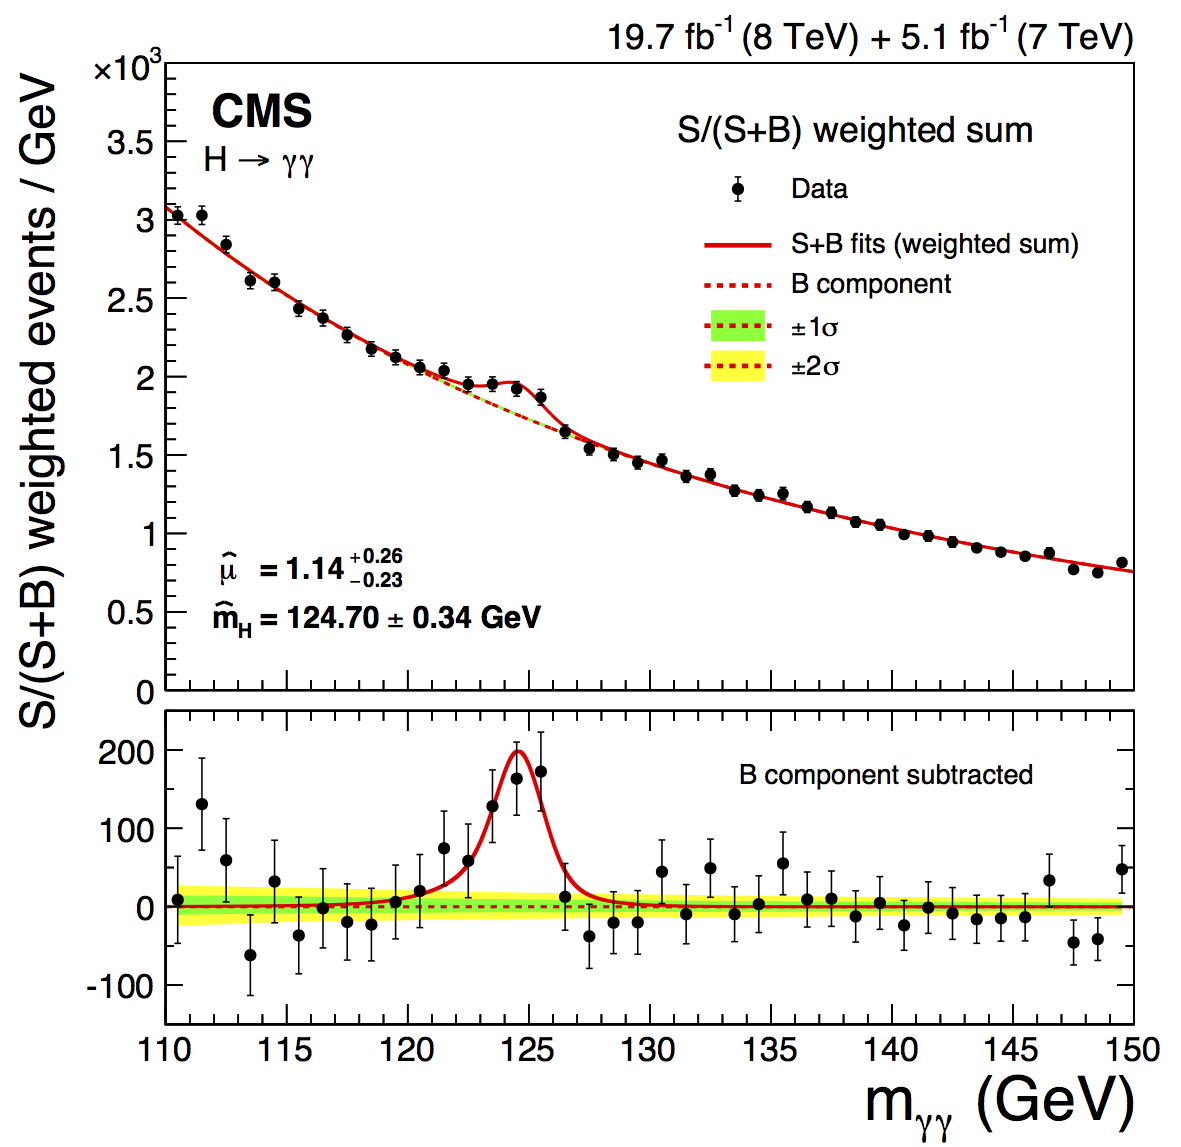
\includegraphics[width=0.6\linewidth]{Figures/higgsmeasurement.png}
\caption{Two photon invariant mass distributions from the CMS detector in 2012~\cite{CMS_Higgs_Discovery}. The peak at $125\GeVcc$ is the Higgs boson.}
\label{fig:higgs}
\end{figure} 


After an upgrade that ended in 2015 the LHC is now capable of producing particle collisions at energies never before achieved. The LHC has also increased its rate of collisions. To be able to gather usable data from these higher energies and collision rates the detectors on the LHC need to be upgraded as well. The Compact Muon Solenoid (CMS), one of the detectors on the LHC, is currently undergoing several upgrades. Chapter~\ref{chap:LHC_CMS} will discuss the details of the LHC and the CMS detector. Chapters~\ref{chap:test} and \ref{chap:sim} will discuss the work I did for the CMS detector outlining the analysis done on new electronics that were installed in the detector during the winter of 2018 as a part of the upgrades

